\documentclass{beamer}
    \usetheme{metropolis} % Use metropolis theme

    \usepackage{graphicx}
    \usepackage[utf8]{inputenc} % Required for inputting international characters
    \usepackage[T1]{fontenc} % Output font encoding for international characters
    \usepackage[none]{hyphenat}
    \usepackage[export]{adjustbox}

    \usepackage[backend=biber,style=nature,natbib=true]{biblatex} 

    \addbibresource{foss.bib} % The filename of the bibliography
        
    \title{Free \& Open Source GIS}
    \date{\today}
    \author{Tereza Pohankova}
    \institute{Department of Geoinformatics, Palacky University Olomouc}
    
    \titlegraphic{{\vspace{6.5cm}
\includegraphics[scale=0.4]{figs/kgilogobarva.png}}}
    
    \begin{document}
     
        \maketitle
        \begin{frame}[allowframebreaks]{FOSS}
            \begin{itemize}
                \item FOSS = Free and Open Source Software
                \item "free" does not primarily point to price (freedom)
                \item openly available for anyone to use, modify and distribute (beware of the licence!)
                \item access to the source code for editing and sharing
                \item promotion of collaboration, transparency, community engagement
                \item one of the first FOSS were Unix (operating system) or TeX (typing)
                \item often supported by commercial companies (IBM, Red Hat, Microsoft)
                
            \end{itemize}

            \begin{figure}
                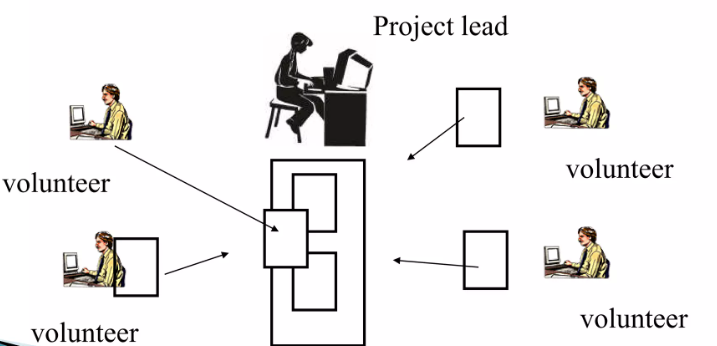
\includegraphics[scale=0.4]{figs/foss_principle.png}
            \end{figure}

            \begin{figure}
                
\includegraphics[scale=0.25]{figs/fossexamples.png}
            \end{figure}

        \end{frame}


        \begin{frame}[allowframebreaks]{Brief History of FOSS}
            \begin{itemize}
                \item 1980s 
                    \begin{itemize}
                        \item limitations until 1970s
                        \item start of the first FOSS projects
                        \item 1984 - GNU by Richard Stallman (core of Unix-based operating systems)
                        \item 1985 - Free Software Foundation (FSF) - supporting visions and goals of all FOSS projects
                        \item 1991 - Linus Torvalds starts Linux projects
                    \end{itemize}

                \item 1990s 
                    \begin{itemize}
                        \item connected to widespread innovations in IT
                        \item Geographical Resources Analysis Support System (GRASS) - originally for US Army
                        \item one of the most known GIS systems, command-line based
                        \item over 300 moduls, OSGeo supported
                        \item 1994 - MapServer
                    \end{itemize}

                \item 21st century 
                    \begin{itemize}
                        \item massive interest in FOSS
                        \item IBM investing in Linux 
                        \item 2001 - Python foundation (Python - one of the most used programming language in FOSS)
                        \item 2001 - GeoServer - sharing and hosting geospatial data
                        \item 2002 - QGIS - multiplatofrm GIS
                        \item 2008 - GitHub - one of the largest platforms for community code contributing
                        \item 2017 - Microsoft becomes the largest contributor in FOSS
                    \end{itemize}
            \end{itemize}
        \end{frame}

        \begin{frame}[allowframebreaks]{Licencing Politics}
            \begin{itemize}
                \item as much openness as possible to everyone
                \item basic principles of FOSS regardless of license:
                    \begin{itemize}
                        \item widespread (and free) possibility of redistribution
                        \item the source code is always shared and possible to modify
                        \item the license must allow the distribution of modified code
                        \item the possibility of dissemination must not discriminate against any person/group
                        \item the license must not restrict use in a specific area
                        \item the rights associated with the program apply to all derivatives
                        \item the rights of the program do not depend on whether the program is part of the distribution of the superior software
                        \item the license must not prevent the use of other programs
                        \item the license must be technologically neutral
                    \end{itemize}
                \item BSD, MIT, Apache, GNU GPL etc.
            \end{itemize}
        \end{frame}

        \begin{frame}[allowframebreaks]{Why is it important?}
            \begin{itemize}
                \item source of innovation, broad ideas
                \item community collaboration
                \item developing of standards
                \item flexibility and quick reparations
            \end{itemize}
        \end{frame}

        \begin{frame}[allowframebreaks]{Organizations in FOSS}
            \begin{itemize}
                \item Free Software Foundation (FSF) \hfill
                    \begin{minipage}[t]{0.35\textwidth}
                        
\includegraphics[scale=0.03]{figs/fsf.png}
                    \end{minipage}
                    \begin{itemize}
                        \item non-profit organization 
                        \item support of rights of FOSS users
                        \item financed by patrons and gifts
                        \item handling legal issues
                    \end{itemize}

               
                
                \item OSGeo \hfill % Adding horizontal space to push logo to the right
                    \begin{minipage}[t]{0.2\textwidth}
                        
\includegraphics[scale=0.07]{figs/osgeo-logo.png}
                    \end{minipage}

                    \begin{itemize}
                        \item \url{https://www.osgeo.org}
                        \item Open Source Geospatial Foundation
                        \item founded 2006
                        \item framework for creating and maintaining geospatial tools and libraries
                        \item fostering global community of users
                        \item QGIS - popular desktop GIS
                        \item GDAL/OGR - library for maintaining raster and vector geodata
                        \item PostGIS - spatial database extension for PostgreSQL - spatial geodata handling and archiving
                        \item PROJ - library for handling spatial reference systems
                        \item FOSS4G - annual global conference for users and developers
                        \item issuing data standards and accessibility
                        \item educational resources
                    \end{itemize}

                    

                \item Open Geospatial Consortium (OGC) \hfill
                    \begin{minipage}[t]{0.25\textwidth}
                        
\includegraphics[scale=0.04]{figs/ogc.png}
                    \end{minipage}

                \begin{itemize}
                    \item established in 1994
                    \item developing and producing open standards
                    \item establish interoperation and seamless data sharing
                    \item developed standards: WMS (Web Map Service), WFS (Web Feature Service), GML (Geography Markup Language), GPKG (GeoPackage)  
                    \item sponsoring pilot projects with industry collaboration global membership community
                \end{itemize}
                
            \end{itemize}
        \end{frame}
        
        \begin{frame}{Notable FOSS GIS Projects}
            \begin{itemize}
                \item \textbf{QGIS (Quantum GIS)}
                    \begin{itemize}
                        \item Desktop GIS with user-friendly interface and extensive plugin support
                        \item Features: vector and raster analysis, geoprocessing, and map composition
                        \item Commonly used in urban planning, environmental monitoring, and non-profit projects
                    \end{itemize}

                \item \textbf{GRASS GIS}
                    \begin{itemize}
                        \item Powerful tool for geospatial data management and spatial modeling
                        \item Strengths in environmental, ecological, and landscape analysis
                        \item Used for land cover analysis, hydrological modeling, and more
                    \end{itemize}
    
                \item \textbf{PostGIS}
                    \begin{itemize}
                        \item Spatial extension for PostgreSQL, a popular open-source relational database
                        \item Provides advanced spatial functions and supports spatial SQL standards
                        \item Used in urban planning, logistics, and telecom for managing large spatial datasets
                    \end{itemize}

                \item \textbf{GDAL/OGR (Geospatial Data Abstraction Library)}
                    \begin{itemize}
                        \item Core library for reading/writing geospatial data formats
                        \item Supports data conversion, warping, and reprojection
                        \item Backbone of many other GIS tools (e.g., QGIS, GRASS)
                    \end{itemize}
                \end{itemize}
            \end{frame}

        \begin{frame}{Web-Based GIS Tools}
            \begin{itemize}
                \item \textbf{MapServer}
                    \begin{itemize}
                        \item Platform for publishing spatial data and creating web-based GIS applications
                        \item Supports OGC standards like WMS and WFS
                        \item Used for government portals, environmental monitoring, and community projects
                    \end{itemize}

                \item \textbf{GeoServer}
                    \begin{itemize}
                        \item Java-based server for sharing and editing geospatial data on the web
                        \item Integrates with data sources like PostGIS and shapefiles
                        \item Popular for complex web mapping and real-time spatial data services
                    \end{itemize}
            \end{itemize}
        \end{frame}

        \begin{frame}{JavaScript Libraries for Web Mapping}
            \begin{itemize}
                \item \textbf{OpenLayers}
                    \begin{itemize}
                        \item JavaScript library for building interactive maps from various sources
                        \item Customizable and mobile-friendly
                        \item Used in web mapping apps and visualizing geographic data in web apps
                    \end{itemize}

                \item \textbf{Leaflet}
                    \begin{itemize}
                        \item Lightweight, easy-to-use JavaScript library for web maps
                        \item Features include interactive maps with layers, markers, and popups
                        \item Often used in lightweight applications, like tourism and local government sites
                    \end{itemize}
            \end{itemize}
        \end{frame}

        \begin{frame}{Specialized Analysis Tools}
            \begin{itemize}
                \item \textbf{PySAL (Python Spatial Analysis Library)}
                    \begin{itemize}
                        \item Python library for spatial data analysis, geostatistics, and econometrics
                        \item Provides clustering, regression, and spatial pattern analysis tools
                        \item Used in academic research, urban studies, and spatial econometrics
                    \end{itemize}
                \item \textbf{GDAL/OGR (Geospatial Data Abstraction Library)}
                    \begin{itemize}
                        \item Core library for reading and writing raster and vector geospatial data formats
                        \item Supports data conversion, warping, and reprojection
                        \item Serves as the backbone of many other GIS tools like QGIS and GRASS
                    \end{itemize}
            \end{itemize}
        \end{frame}

                
        \nocite{*}
        \frame[shrink=30]{\printbibliography[heading=bibintoc]}
    \end{document}